\documentclass[14pt]{beamer}
\usetheme{metropolis}
\usepackage{appendixnumberbeamer}
\usepackage{booktabs}
\usepackage{amsmath}
\usepackage[scale=2]{ccicons}
\usepackage{fontawesome}
\usepackage{fontspec}
%\usepackage{pgfplots}
%\usepgfplotslibrary{dateplot}
\usepackage{xspace}
\usepackage{graphicx}
\usepackage{tikz}
\usepackage{fontawesome}
\usepackage{setspace}
%\newfontfamily{\FA}{FontAwesome Regular}	
\def\twitter{{\FA \faTwitter}}
\def\github{{\FA \faGithub}}
\def\www{{\FA \faGlobe}}
\newcommand{\themename}{\textbf{\textsc{metropolis}}\xspace}
%\newfontfamily{\FA}{FontAwesome Regular}	
\setbeamerfont{frametitle}{size=\large}
\title{Lasso and capture-recapture}
\subtitle{Olivier Gimenez and Ian Renner}
%\date{\today}
\date{}
%\institute{{\small \twitter\ oaggimenez \www\ oliviergimenez.github.io}}
\titlegraphic{\hfill\includegraphics[height=1.1cm]{CNRSinter-Q_p.jpg}}

\begin{document}

\maketitle

\section{Introduction}

\usebackgroundtemplate{
\begin{picture}(100,280)
\includegraphics[width=1.1\paperwidth]{trip_opacity.jpg}
\end{picture}
}%

\begin{frame}{What is this about?}

\begin{itemize}
\item Explain variation in abundance and survival
\item Capture-recapture models are often used
\item Survival models with imperfect detection
\item With technology, come many variables
\item Often do not know which ones (not) to include
\end{itemize}

\end{frame}

\setbeamertemplate{background canvas}[default]

\begin{frame}[fragile]{What are the issues?}

Many, possibly correlated, covariates

{
  \begin{figure}
    \centering
    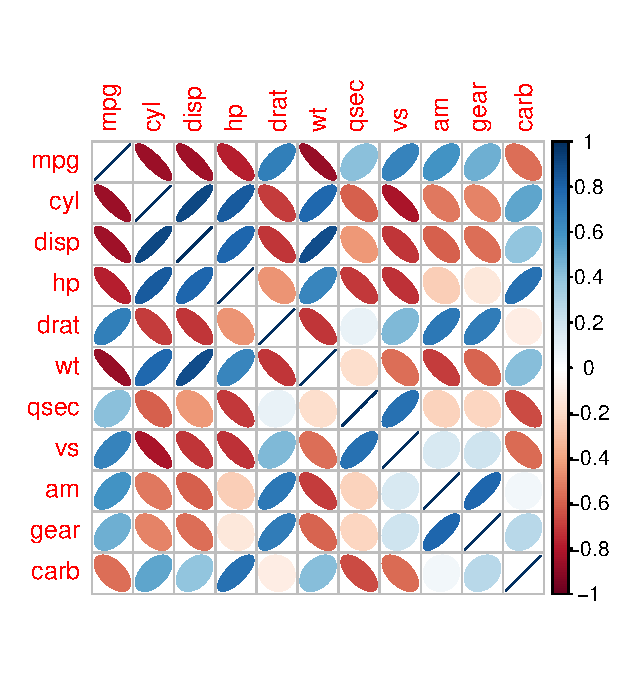
\includegraphics[width = 0.3\textwidth]{coor_matrix.eps}
%    \caption{Awesome figure}
  \end{figure}
}

Correlation $\implies$ numerical instability

Many covariates $\implies$ $\searrow$ precision and predictability

\end{frame}

\begin{frame}[fragile]{What we usually do}

Think hard about which covariates to consider

Select covariates using:
\begin{itemize}
\item AIC or stepwise procedure
\item DIC, SSVS, RJMCMC
\end{itemize}

\textbf{This talk:} shrink and select model coefficients

\end{frame}

\section{Theory}

\begin{frame}[fragile]{The reference - free book!}

{
  \begin{figure}
    \centering
    \includegraphics[width = 0.45\textwidth]{sls.jpg}
%    \caption{Awesome figure}
  \end{figure}
}

\end{frame}

\usebackgroundtemplate{
\begin{picture}(100,280)
\includegraphics[width=1.1\paperwidth]{ridge_opacity.jpg}
\end{picture}
}%

\begin{frame}[fragile]{It all starts with the ridge regression}

Maximize likelihood, penalize magnitude of coeff.

$\widehat{\boldsymbol{\beta}} = \text{argmax} \; L(\boldsymbol{\beta})$ subject to $\displaystyle{\sum_{j=1}^{p}{ \beta_j^2}} < c$

\end{frame}

\begin{frame}[fragile]{It all starts with the ridge regression}

{\color{blue}Maximize likelihood}, penalize magnitude of coeff.

{\color{blue}$\widehat{\boldsymbol{\beta}} = \text{argmax} \; L(\boldsymbol{\beta})$} subject to $\displaystyle{\sum_{j=1}^{p}{ \beta_j^2}} < c$

\end{frame}

\begin{frame}[fragile]{It all starts with the ridge regression}

Maximize likelihood, {\color{blue}penalize magnitude of coeff.}

$\widehat{\boldsymbol{\beta}} = \text{argmax} \; L(\boldsymbol{\beta})$ subject to {\color{blue}$\displaystyle{\sum_{j=1}^{p}{ \beta_j^2}} < c$}

\end{frame}

\setbeamertemplate{background canvas}[default]

\begin{frame}[fragile]{Lasso $=$ \small{Least Absolute \alert{Shrinkage} and \alert{Selection} Operator}}

Change the constraint: $\ell^2$ vs. $\ell^1$ norm

$\widehat{\boldsymbol{\beta}} = \text{argmax} \; L(\boldsymbol{\beta})$ subject to $\displaystyle{\sum_{j=1}^{p}{\lvert \beta_j \rvert}} < c$

\end{frame}

\begin{frame}[fragile]{Lasso vs. ridge regression, graphically}

{
  \begin{figure}
    \centering
    \includegraphics[width = 1\textwidth]{lasso2.jpeg}
%    \caption{Awesome figure}
% Shrunken feasible regions for L1/LASSO penalized regression parameters (left) and L2/ridge penalized regression parameters (right). Image courtesy Patrick Hall, Tomas Nykodym, and the H2O.ai team.
  \end{figure}
}

\end{frame}

\begin{frame}[fragile]{Lasso: maximizing penalized likelihood}

$\widehat{\boldsymbol{\beta}} = \text{argmax} \; L(\boldsymbol{\beta})$ subject to $\displaystyle{\sum_{j=1}^{p}{\lvert \beta_j \rvert}} < c$

Constrained optimization not easy

Rewrite the problem with Lagrange multipliers

$\widehat{\boldsymbol{\beta}} = {\text{argmax} \; L(\boldsymbol{\beta})} + \lambda \displaystyle{\sum_{j=1}^{p}{\lvert \beta_j \rvert}}$

Adaptive lasso penalty to achieve oracle properties

\end{frame}

\begin{frame}[fragile]{Lasso: maximizing penalized likelihood}

$\widehat{\boldsymbol{\beta}} = \text{argmax} \; L(\boldsymbol{\beta})$ subject to $\displaystyle{\sum_{j=1}^{p}{\lvert \beta_j \rvert}} < c$

Constrained optimization not easy

Rewrite the problem with Lagrange multipliers

$\widehat{\boldsymbol{\beta}} = \text{argmax} \; \alert{L(\boldsymbol{\beta})} + \lambda \displaystyle{\sum_{j=1}^{p}{\lvert \beta_j \rvert}}$; \alert{capture-recapt. lik.}

Adaptive lasso penalty to achieve oracle properties

\end{frame}

\begin{frame}[fragile]{Capture--recapture likelihood}

\begin{itemize}
\item 1s and 0s for detections and non-detections
\item For example, animal $i$ may be $h_i = 101$
\item Denote $\phi^t$ survival prob between $t$ and $t+1$ and $p^t$ recapture prob at $t$ 
\item Contribution of animal $i$ to likelihood is $\Pr(h_i) = \phi^1 (1-p^2) \phi^2 p^3$
\item $\text{logit}(\phi^t) = \beta_0 + \beta_1 x_1^t + \ldots + \beta_{K} x^t_{K}$
\item Likelihood is $\displaystyle{\prod_i \Pr(h_i)}$ for all animals $i$
\end{itemize}

\end{frame}

\begin{frame}[fragile]{How to choose the penalty term $\lambda$?}

\begin{itemize}
\item Usually, cross-validation techniques
\item Build a grid of values for $\lambda$
\item Repeat optimization for each value of the grid
\item Pick $\lambda$ corresponding to model with lowest BIC
\end{itemize}

\end{frame}

\setbeamertemplate{background canvas}[default]

\section{Simulations}

%\usebackgroundtemplate{
%%\begin{picture}(50,265)
%%\includegraphics[width=0.6\paperwidth]{r_logo_opacity.png}
%\includegraphics[width=0.9\paperwidth,height=1\paperheight]{r_logo_opacity.png}
%%\end{picture}
%}%

\begin{frame}[fragile]{Setting: Capture-recapture model}

\begin{itemize}
\item Sample size: 15 occasions with 15 new ind.
\item Detection is 0.9, mean survival is 0.8
\item Covariates: $X_1 \sim N(\alert{-0.6},\sigma=1)$, $X_2 \sim N(\alert{0},\sigma=1)$
\item Apply Lasso; fit 4 models, compare with AIC
\item Repeat 100 times
\end{itemize}


\end{frame}

\begin{frame}[fragile]{Simulation results}

\begin{itemize}
\item Lasso selects correct model ($X_1$ only) $80\%$ 
\item Comparable to variable selection using AIC
\item Further simulations show similar results
\end{itemize}

\end{frame}


\section{Application}

\begin{frame}[fragile]{White storks wintering in Sahel}

Capture-recapture data over 16 years

Rainfall was measured at 10 meteo stations in Sahel

{
  \begin{figure}
    \centering
    \includegraphics[width = 0.15\textwidth]{Ringed_white_stork.jpg}
 %   \caption{Awesome figure}
  \end{figure}

}

Is adult white stork survival affected by rainfall?

$\text{logit}(\phi^t) = \beta_0 + \beta_1 x_1^t + \ldots + \beta_{10} x_{10}^t$

Do we need to consider $2^{10}$ candidate models?

\end{frame}

\begin{frame}[fragile]{Choosing the Lasso penalty using BIC}

{
  \begin{figure}
    \centering
    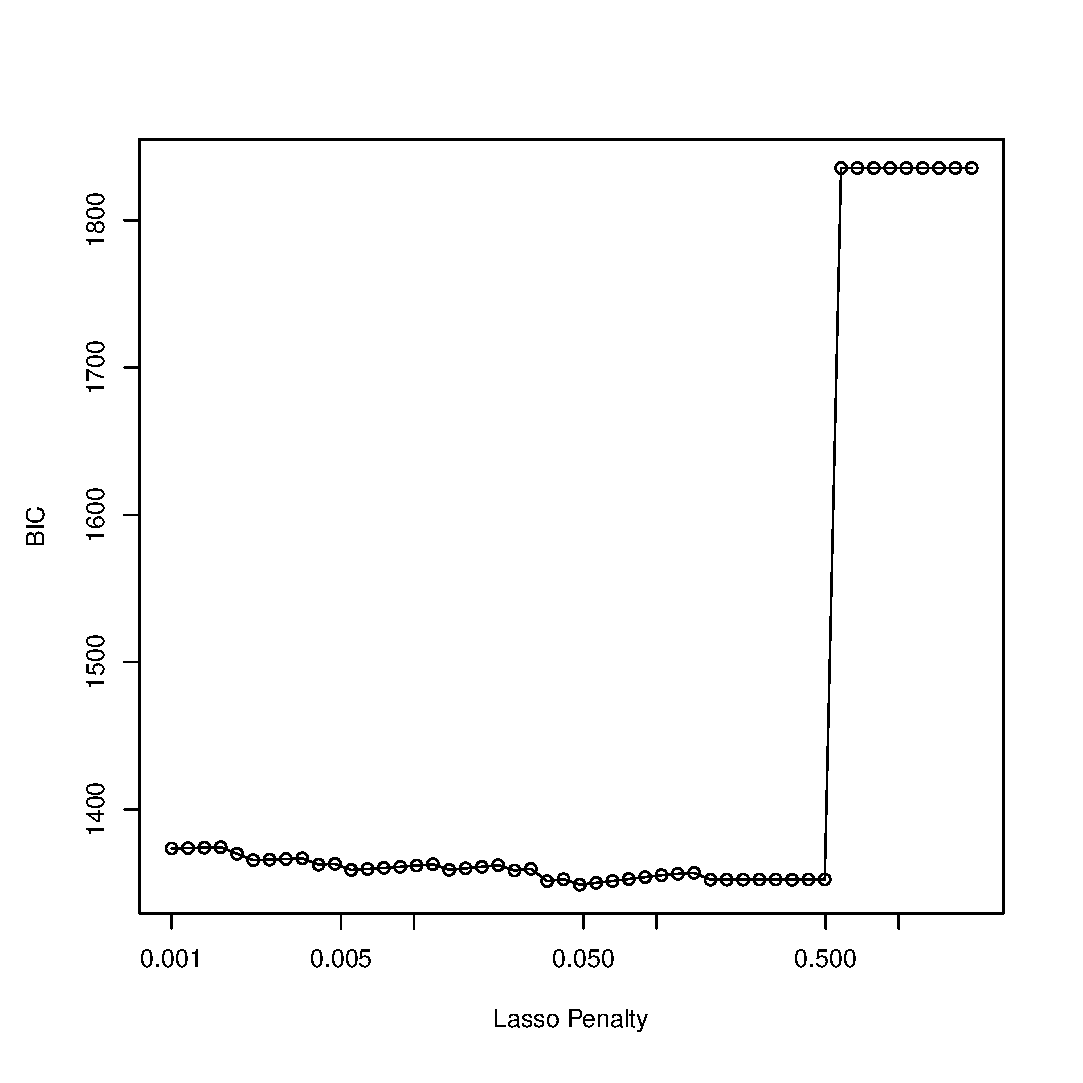
\includegraphics[width = 0.7\textwidth]{bic.eps}
  %  \caption{Awesome figure}
  \end{figure}

}

\end{frame}

\begin{frame}[fragile]{Exploring regularization path}

{
  \begin{figure}
    \centering
    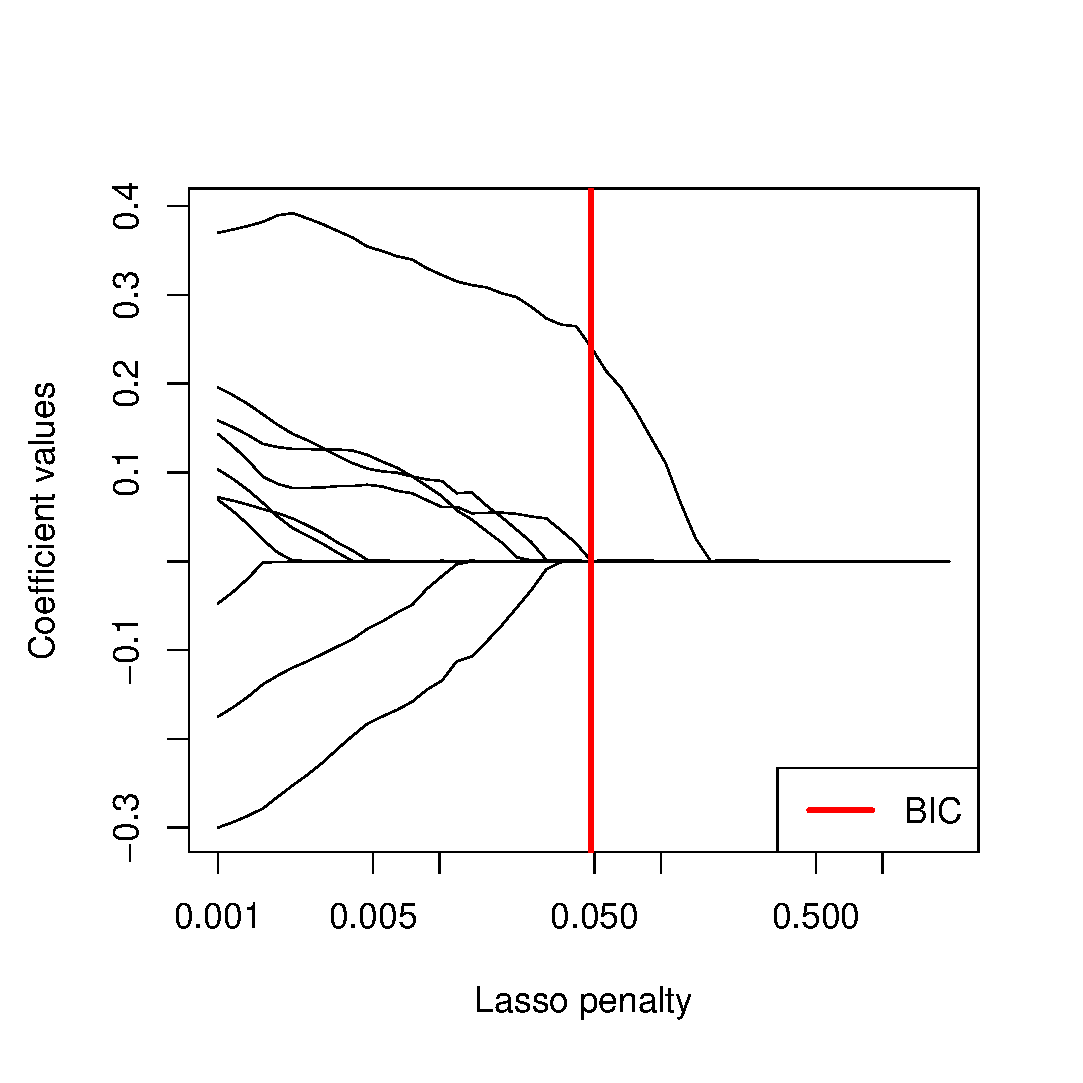
\includegraphics[width = 0.7\textwidth]{path.eps}
   % \caption{Awesome figure}
  \end{figure}

}

\end{frame}

\begin{frame}{Rainfall effect at all weather stations}
\begin{small}
  \begin{table}
    %\caption{Largest cities in the world (source: Wikipedia)}
    \begin{tabular}{@{} lr @{}}
      \toprule
      Station & Estimate\\
      \midrule
      Diourbel & 7.47 x $10^{-5}$\\
      Gao & -2.99 x $10^{-5}$\\
      Kayes & 1.3 x $10^{-4}$\\
      \alert{Kita} & \alert{0.24} \\
      Maradi & -1.3 x $10^{-4}$\\
      Mopti & 3.5 x $10^{-4}$\\
      Ouahigouya & -5.9 x $10^{-5}$\\
      Segou & 1.7 x $10^{-5}$\\
      Tahoua & 1.2 x $10^{-4}$\\
      Tombouctou & -2.3 x $10^{-4}$\\
      \bottomrule
    \end{tabular}
  \end{table}
\end{small}
\end{frame}


\section{Conclusions and perspectives}

\begin{frame}{Conclusions and perspectives}

\begin{itemize}
\item From selecting variables to \alert{shrinking} estimates
\item Penalized likelihood easy to implement
\item Ongoing work with Bayesian flavor
\end{itemize}

\end{frame}

\begin{frame}[standout]
  Questions
\end{frame}

\end{document}
